\documentclass[11pt, a4paper]{article}
\usepackage[utf8]{inputenc}
\usepackage[margin=1in]{geometry} %Sets proper 1-inch margins. 
\usepackage{amsmath} %Only load this if you are using math/equations.
\usepackage{graphicx} %Only need to call this if inserting images.
\usepackage{caption} %Only need to call this if inserting captions.
\usepackage{float} %Allows the use of the [H] specifier. 
\usepackage[colorlinks,citecolor=blue,linkcolor=blue,urlcolor=blue]{hyperref} %Allows for the embedding of urls. 
\usepackage{setspace}
\usepackage{blindtext}

\pagenumbering{arabic}

\usepackage{fancyhdr}

\pagestyle{fancy}
\fancyhf{}
\rhead{Jonah Edmundson \\ 2023}
\lhead{\thepage}

\newcommand{\comment}[1]{}

\usepackage{Sweave}
\begin{document}
\Sconcordance{concordance:regression.tex:regression.Rnw:%
1 22 1 1 0 20 1 1 12 1 8 4 1 1 5 3 0 1 1 41 0 1 3 1 4 3 0 1 10 1 0 1 2 %
2 1 1 11 1 1 1 5 14 0 1 2 4 1 1 4 2 2 3 0 1 1 8 0 1 2 6 1 1 5 1 1 1 5 3 %
0 1 1 40 0 1 3 1 5 3 0 1 10 1 0 1 2 2 1 1 11 1 1 1 6 14 0 1 2 4 1 1 4 1 %
2 9 1 1 5 1 3 1 1 1 5 3 0 1 1 13 0 1 5 2 0 1 11 1 0 1 2 9 1 1 6 1 4 49 %
0 1 2 1 1 1 5 3 0 1 11 1 0 1 2 7 1 1 8 25 0 1 3 2 0 1 10 1 0 1 2 6 1 1 %
6 15 0 1 2 1 1 1 10 1 4 3 0 1 10 1 0 1 2 7 1 1 4 11 0 1 2 1 1 1 4 3 0 1 %
11 1 0 1 2 7 1 1 4 3 0 1 1 12 0 1 2 1 4 3 0 1 10 1 0 1 2 10 1 1 3 3 0 1 %
10 4 0 1 2 18 1 1 5 38 0 1 3 1 5 3 0 1 10 1 0 1 2 2 1 1 5 14 0 1 2 6 1 %
1 6 1 4 49 0 1 2 1 1 1 5 3 0 1 11 1 0 1 2 7 1 1 8 25 0 1 3 2 0 1 10 1 0 %
1 2 4 1 1 5 14 0 1 2 1 1 1 10 1 4 3 0 1 10 1 0 1 2 7 1 1 3 11 0 1 2 1 1 %
1 4 3 0 1 11 1 0 1 2 7 1 1 3 3 0 1 1 12 0 1 2 1 4 3 0 1 10 1 0 1 2 10 1 %
1 3 3 0 1 10 4 0 1 2 18 1 1 3 1 2 7 1 1 3 1 2 9 1 1 3 1 2 10 1 1 30 3 0 %
1 1 6 0 1 1 14 0 1 1 2 0 1 1 6 0 1 1 14 0 1 10 1 0 1 2 11 1 1 2 3 0 1 %
15 1 0 1 2 11 1 1 7 3 0 1 2 4 0 1 3 1 0 1 2 12 1 1 14 7 0 1 1 14 0 1 3 %
1 0 1 2 9 1}


\begin{center}
\Large{\textsc{Regression Analysis}}
\par
\normalsize{\textsc{for}}
\par
\large{\textsc{Kelowna Weather-Crash Project}}
\end{center}


\vspace{0.917 pc} %Creates a paragraph line break. 

\tableofcontents



\pagebreak
\section{Predicting Number of Crashes}





\subsection{Multiple Linear Regression}

\begin{Schunk}
\begin{Soutput}
With backwards and forward selection using 'step()':
\end{Soutput}
\begin{Soutput}
Call:
lm(formula = crashes ~ month + day + relhum + precip + wind.dir + 
    wind.spd + visibility, data = train, x = TRUE, y = TRUE)

Residuals:
    Min      1Q  Median      3Q     Max 
-82.657 -17.998   0.226  19.747 166.522 

Coefficients:
               Estimate Std. Error t value Pr(>|t|)    
(Intercept)    248.3339    39.4690   6.292 1.06e-09 ***
monthAUGUST     21.4353     9.7515   2.198 0.028671 *  
monthDECEMBER   40.8051    11.7764   3.465 0.000604 ***
monthFEBRUARY   41.5961    10.6586   3.903 0.000117 ***
monthJANUARY    57.8888    12.1759   4.754 3.04e-06 ***
monthJULY       30.3272     9.1724   3.306 0.001055 ** 
monthJUNE       26.1346     8.5632   3.052 0.002468 ** 
monthMARCH      13.7881     8.8537   1.557 0.120403    
monthMAY        18.7967     8.4966   2.212 0.027670 *  
monthNOVEMBER   35.4994    11.1850   3.174 0.001654 ** 
monthOCTOBER    35.2250     9.7665   3.607 0.000361 ***
monthSEPTEMBER  23.1569     8.6477   2.678 0.007801 ** 
dayMONDAY      -24.6982     6.3687  -3.878 0.000128 ***
daySATURDAY    -44.2414     6.3844  -6.930 2.41e-11 ***
daySUNDAY      -64.2965     6.3471 -10.130  < 2e-16 ***
dayTHURSDAY     -8.4554     6.3670  -1.328 0.185142    
dayTUESDAY      -9.6025     6.3569  -1.511 0.131908    
dayWEDNESDAY    -9.2981     6.3458  -1.465 0.143858    
relhum          -0.8501     0.3610  -2.355 0.019151 *  
precip           0.9424     0.4563   2.065 0.039718 *  
wind.dir         1.9817     0.9429   2.102 0.036376 *  
wind.spd        -2.6151     1.0352  -2.526 0.012023 *  
visibility      -5.0721     1.6142  -3.142 0.001838 ** 
---
Signif. codes:  0 ‘***’ 0.001 ‘**’ 0.01 ‘*’ 0.05 ‘.’ 0.1 ‘ ’ 1

Residual standard error: 30.97 on 313 degrees of freedom
Multiple R-squared:  0.4441,	Adjusted R-squared:  0.405 
F-statistic: 11.37 on 22 and 313 DF,  p-value: < 2.2e-16
\end{Soutput}
\end{Schunk}

\begin{Schunk}
\begin{Soutput}
MLR MSE: 990.7888
\end{Soutput}
\end{Schunk}
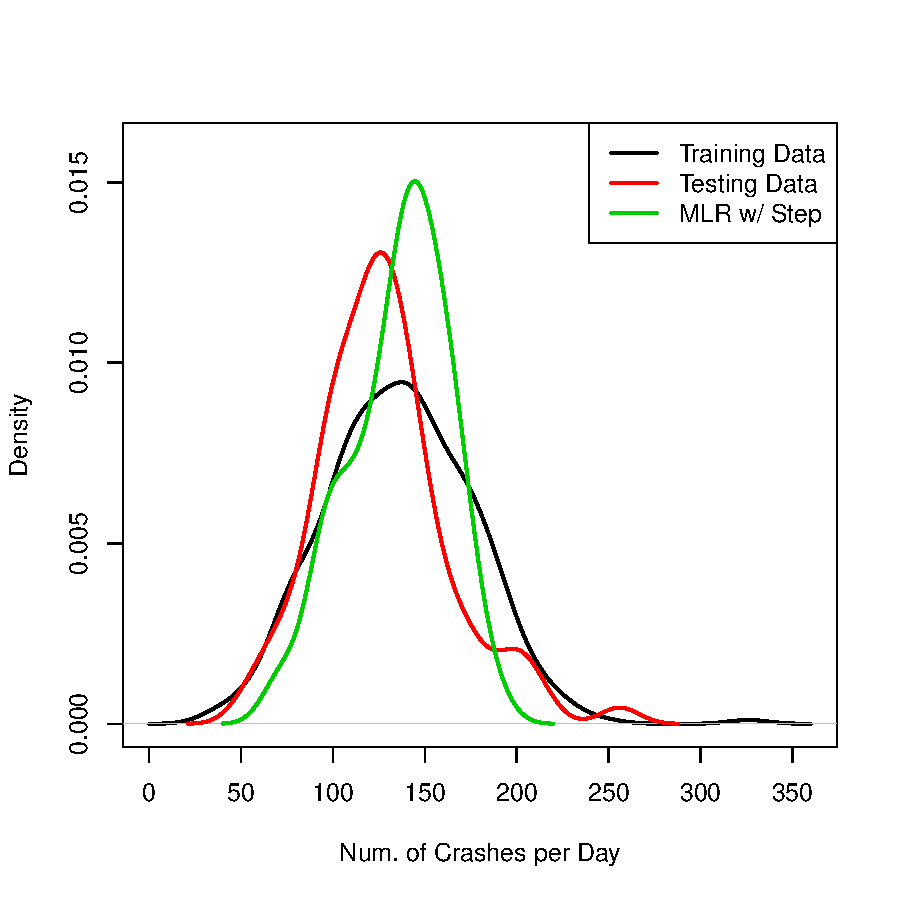
\includegraphics{regression-004}





\begin{Schunk}
\begin{Soutput}
Consistent Model Specification Test
Parametric null model: lm(formula = crashes ~ month + day + temp + relhum +
                          precip + wind.dir + wind.spd + visibility + pressure,
                          data = train, x = TRUE, y = TRUE)
Number of regressors: 9
IID Bootstrap (399 replications)

Test Statistic ‘Jn’: 2.125212	P Value: 0.0075188 **
---
Signif. codes:  0 '***' 0.001 '**' 0.01 '*' 0.05 '.' 0.1 ' ' 1
Null of correct specification is rejected at the 1% level
\end{Soutput}
\end{Schunk}

\pagebreak

\noindent\textbf{MLR Model Diagnostics:}

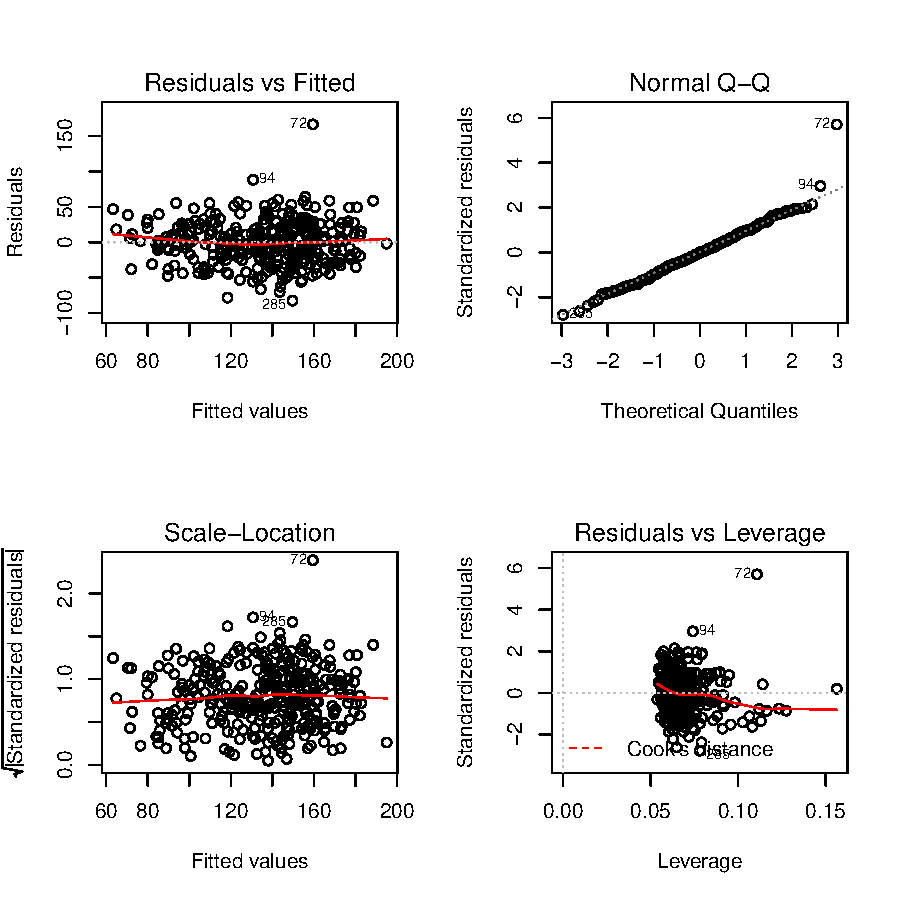
\includegraphics{regression-007}

\begin{Schunk}
\begin{Soutput}
Point 72:
\end{Soutput}
\begin{Soutput}
                   linker    month      day     temp relhum precip wind.dir
72 2017 NOVEMBER THURSDAY NOVEMBER THURSDAY 3.244167   88.5   18.7 19.20085
   wind.spd visibility pressure crashes victims parked HWY97 HARVEY HWY33
72 11.43333   13.09917 95.80075     326     147     70    33     10    21
   GORDON year
72     14 2017
\end{Soutput}
\end{Schunk}




\pagebreak
\subsection{MLR Outliers Removed}



\begin{Schunk}
\begin{Soutput}
With backwards and forward selection using 'step()':
\end{Soutput}
\begin{Soutput}
Call:
lm(formula = crashes ~ month + day + relhum + wind.dir + wind.spd + 
    visibility, data = train, x = TRUE, y = TRUE)

Residuals:
    Min      1Q  Median      3Q     Max 
-77.259 -18.539  -1.277  19.245  87.761 

Coefficients:
               Estimate Std. Error t value Pr(>|t|)    
(Intercept)    226.0928    36.2392   6.239 1.43e-09 ***
monthAUGUST     22.8495     9.2334   2.475 0.013866 *  
monthDECEMBER   34.9678    10.6659   3.278 0.001161 ** 
monthFEBRUARY   35.5950     9.4245   3.777 0.000190 ***
monthJANUARY    51.1036    10.7197   4.767 2.87e-06 ***
monthJULY       33.1438     8.5406   3.881 0.000127 ***
monthJUNE       28.8859     8.0154   3.604 0.000365 ***
monthMARCH      11.2022     8.2851   1.352 0.177321    
monthMAY        22.0047     7.8938   2.788 0.005635 ** 
monthNOVEMBER   22.9119    10.2012   2.246 0.025401 *  
monthOCTOBER    30.8668     9.0629   3.406 0.000746 ***
monthSEPTEMBER  21.7934     8.1734   2.666 0.008066 ** 
dayMONDAY      -25.1623     6.0412  -4.165 4.03e-05 ***
daySATURDAY    -44.6592     6.0515  -7.380 1.44e-12 ***
daySUNDAY      -64.3616     6.0213 -10.689  < 2e-16 ***
dayTHURSDAY    -12.4378     6.0778  -2.046 0.041549 *  
dayTUESDAY      -9.8105     6.0302  -1.627 0.104769    
dayWEDNESDAY    -9.6708     6.0203  -1.606 0.109202    
relhum          -0.5819     0.2980  -1.953 0.051731 .  
wind.dir         2.1891     0.8938   2.449 0.014864 *  
wind.spd        -3.2337     0.9844  -3.285 0.001136 ** 
visibility      -4.3765     1.5345  -2.852 0.004632 ** 
---
Signif. codes:  0 ‘***’ 0.001 ‘**’ 0.01 ‘*’ 0.05 ‘.’ 0.1 ‘ ’ 1

Residual standard error: 29.38 on 313 degrees of freedom
Multiple R-squared:  0.4638,	Adjusted R-squared:  0.4278 
F-statistic: 12.89 on 21 and 313 DF,  p-value: < 2.2e-16
\end{Soutput}
\end{Schunk}

\begin{Schunk}
\begin{Soutput}
MLR MSE: 1029.308
\end{Soutput}
\end{Schunk}
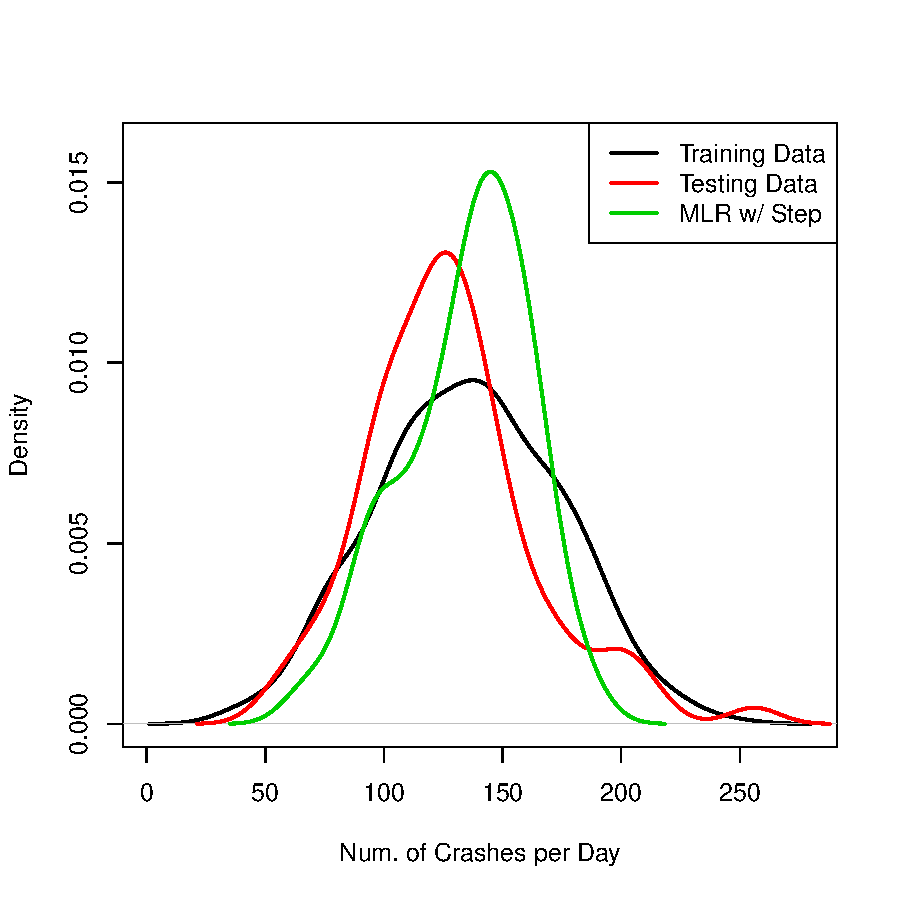
\includegraphics{regression-011}





\begin{Schunk}
\begin{Soutput}
Consistent Model Specification Test
Parametric null model: lm(formula = crashes ~ month + day + relhum + wind.dir +
                          wind.spd + visibility, data = train, x = TRUE, y =
                          TRUE)
Number of regressors: 9
IID Bootstrap (399 replications)

Test Statistic ‘Jn’: 1.956675	P Value: 0.0075188 **
---
Signif. codes:  0 '***' 0.001 '**' 0.01 '*' 0.05 '.' 0.1 ' ' 1
Null of correct specification is rejected at the 1% level
\end{Soutput}
\end{Schunk}


\pagebreak
\noindent\textbf{MLR Model Diagnostics:}

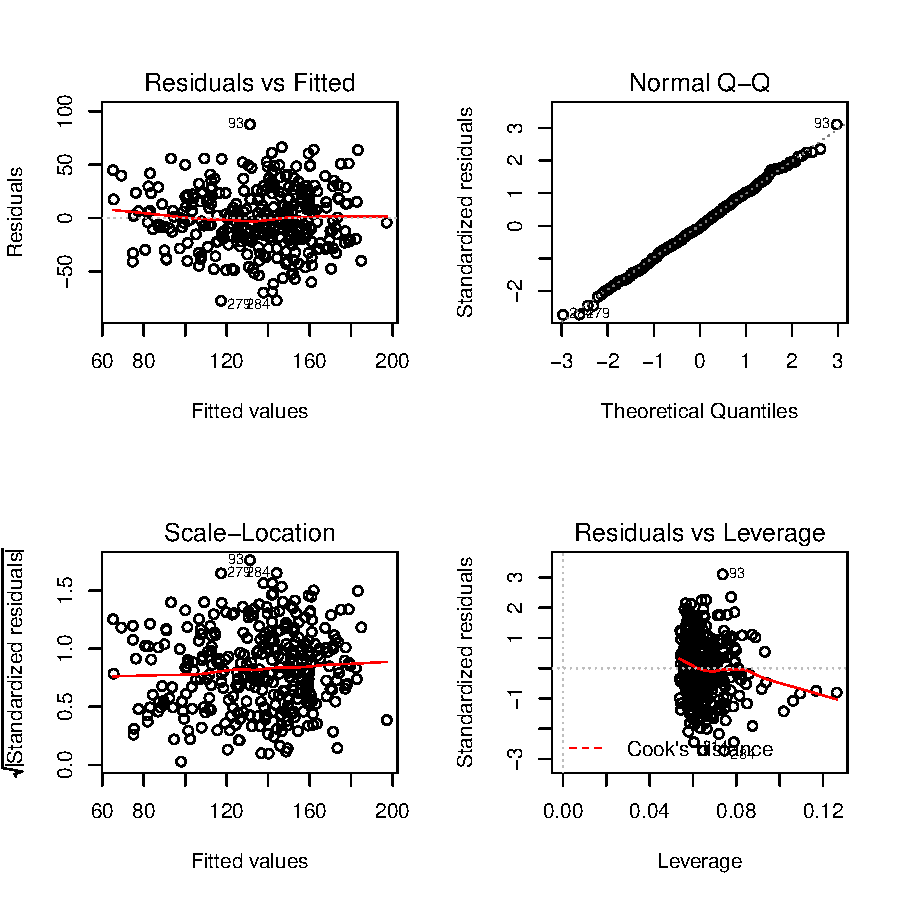
\includegraphics{regression-014}






\pagebreak
\subsection{LASSO Variable Selection}
%\noindent\textbf{LASSO Variable Selection}

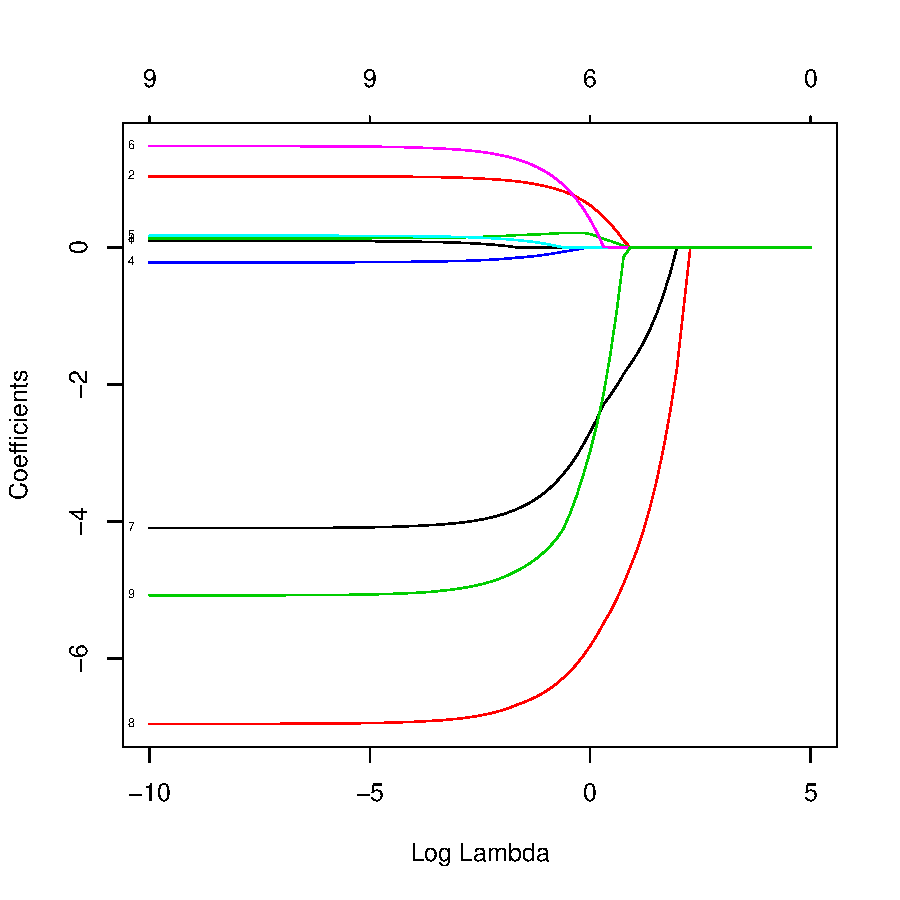
\includegraphics{regression-015}


\begin{Schunk}
\begin{Soutput}
Value of lambda that results in the lowest MSE: 1.833195
\end{Soutput}
\begin{Soutput}
10 x 1 sparse Matrix of class "dgCMatrix"
                      s0
(Intercept) 316.42924787
month         .         
day           0.23352977
temp          0.06176113
relhum        .         
precip        .         
wind.dir      .         
wind.spd     -2.01652421
visibility   -5.12835456
pressure     -0.91108125
\end{Soutput}
\begin{Soutput}
MLR w/ LASSO MSE: 1334.424
\end{Soutput}
\end{Schunk}
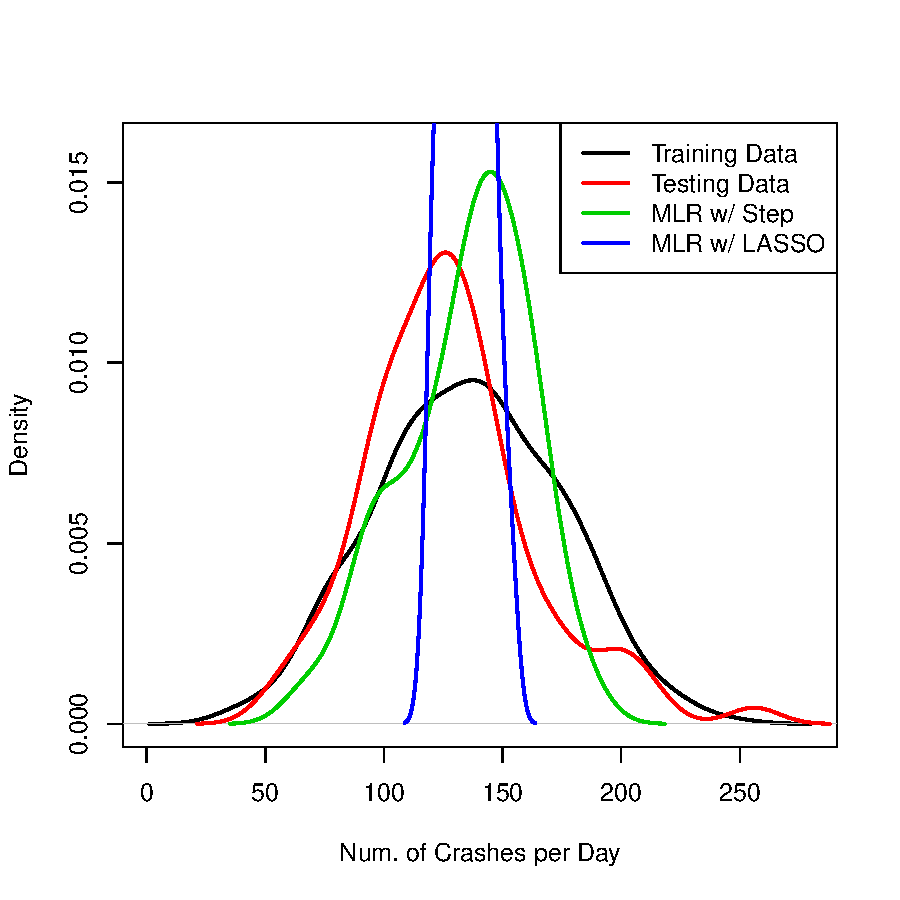
\includegraphics{regression-016}


This is clearly a terrible fit.....




\pagebreak
\subsection{Generalized Linear Model}


\begin{Schunk}
\begin{Soutput}
Call:
glm(formula = crashes ~ month + day + temp + relhum + precip + 
    wind.dir + wind.spd + visibility + pressure, family = gaussian(link = "identity"), 
    data = train)

Deviance Residuals: 
    Min       1Q   Median       3Q      Max  
-79.335  -18.853   -0.679   19.692   88.901  

Coefficients:
               Estimate Std. Error t value Pr(>|t|)    
(Intercept)    791.9625   565.5173   1.400 0.162387    
monthAUGUST     28.1143    14.2525   1.973 0.049431 *  
monthDECEMBER   38.0453    13.6585   2.785 0.005674 ** 
monthFEBRUARY   34.8072    14.6491   2.376 0.018106 *  
monthJANUARY    52.9286    14.6668   3.609 0.000359 ***
monthJULY       38.2162    14.7552   2.590 0.010050 *  
monthJUNE       31.9660    11.8956   2.687 0.007594 ** 
monthMARCH      10.5997     9.7818   1.084 0.279377    
monthMAY        23.4757    10.4261   2.252 0.025046 *  
monthNOVEMBER   25.7166    11.7240   2.193 0.029014 *  
monthOCTOBER    34.9887     9.5613   3.659 0.000297 ***
monthSEPTEMBER  26.9859    10.7824   2.503 0.012837 *  
dayMONDAY      -24.3617     6.1856  -3.938 0.000101 ***
daySATURDAY    -44.0734     6.0752  -7.255 3.25e-12 ***
daySUNDAY      -63.9712     6.0884 -10.507  < 2e-16 ***
dayTHURSDAY    -12.5281     6.1086  -2.051 0.041118 *  
dayTUESDAY      -9.7347     6.1057  -1.594 0.111870    
dayWEDNESDAY    -9.6339     6.0622  -1.589 0.113041    
temp            -0.5824     1.0183  -0.572 0.567779    
relhum          -0.8393     0.3532  -2.376 0.018089 *  
precip           0.4340     0.4469   0.971 0.332244    
wind.dir         2.1701     0.8995   2.413 0.016416 *  
wind.spd        -3.5396     1.0086  -3.510 0.000515 ***
visibility      -4.1926     1.5441  -2.715 0.006993 ** 
pressure        -5.6648     5.8171  -0.974 0.330908    
---
Signif. codes:  0 ‘***’ 0.001 ‘**’ 0.01 ‘*’ 0.05 ‘.’ 0.1 ‘ ’ 1

(Dispersion parameter for gaussian family taken to be 865.032)

    Null deviance: 503970  on 334  degrees of freedom
Residual deviance: 268160  on 310  degrees of freedom
AIC: 3242.2

Number of Fisher Scoring iterations: 2
\end{Soutput}
\end{Schunk}


\begin{Schunk}
\begin{Soutput}
GLM MSE: 974.3266
\end{Soutput}
\end{Schunk}
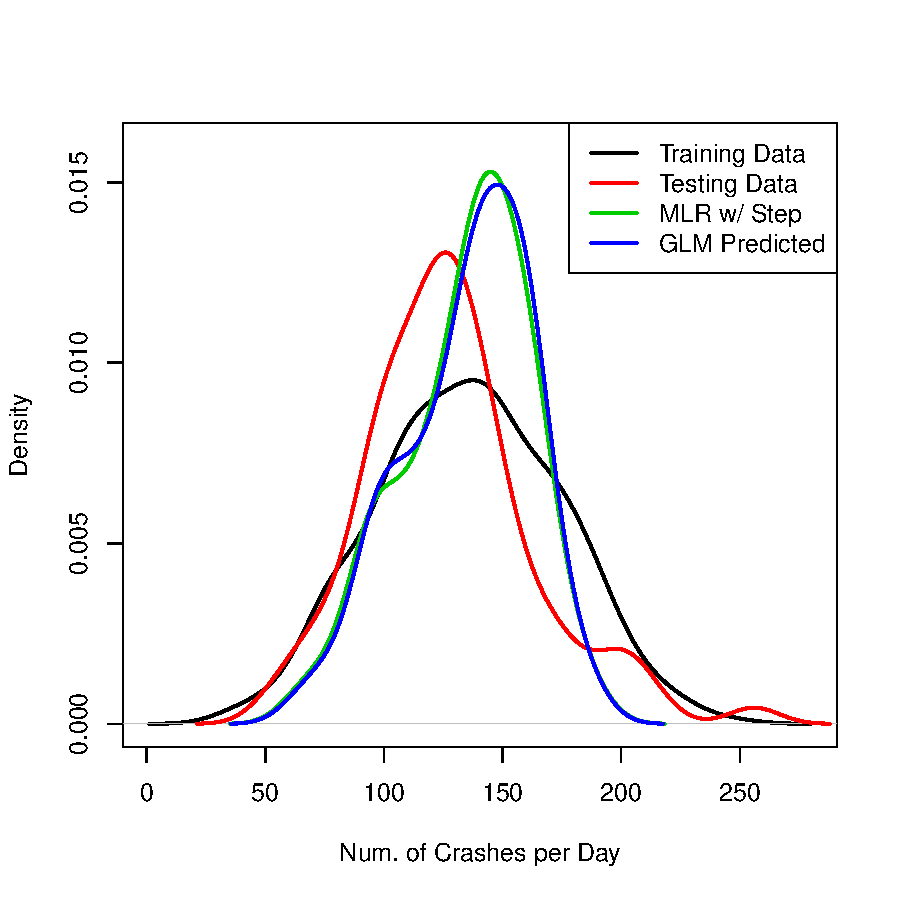
\includegraphics{regression-019}





\pagebreak
\subsection{Non-parametric Approach}

\begin{Schunk}
\begin{Soutput}
Kernel Regression Significance Test
Type I Test with IID Bootstrap (399 replications, Pivot = TRUE, joint = FALSE)
Explanatory variables tested for significance:
month (1), day (2), temp (3), relhum (4), precip (5), wind.dir (6), wind.spd (7), visibility (8), pressure (9)

                 month       day     temp   relhum  precip wind.dir wind.spd
Bandwidth(s): 0.916666 0.4419936 9.705523 12.39832 6428386 20379937 14.35713
              visibility pressure
Bandwidth(s):    6167572  6886070

Individual Significance Tests
P Value: 
month      0.0075188 ** 
day        < 2.22e-16 *** 
temp       0.0175439 * 
relhum     0.6892231  
precip     0.2706767  
wind.dir   0.0350877 * 
wind.spd   < 2.22e-16 *** 
visibility 0.0100251 * 
pressure   0.1027569 
---
Signif. codes:  0 '***' 0.001 '**' 0.01 '*' 0.05 '.' 0.1 ' ' 1
\end{Soutput}
\begin{Soutput}
Non-parametric MSE: 1203.843
\end{Soutput}
\end{Schunk}
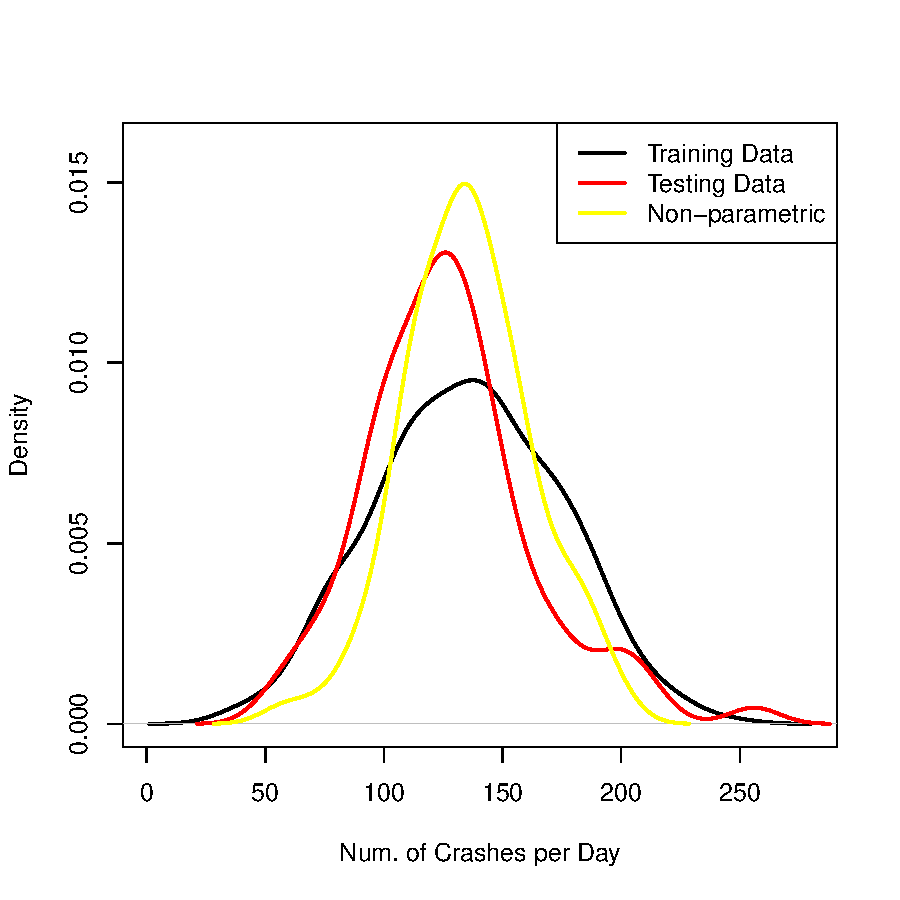
\includegraphics{regression-020}




\pagebreak
\subsection{Decision Tree}

\begin{Schunk}
\begin{Soutput}
Regression tree:
tree(formula = crashes ~ month + day + temp + relhum + precip + 
    wind.dir + wind.spd + visibility + pressure, data = train)
Variables actually used in tree construction:
[1] "day"        "month"      "temp"       "wind.spd"   "pressure"  
[6] "visibility" "precip"    
Number of terminal nodes:  15 
Residual mean deviance:  705.1 = 225600 / 320 
Distribution of residuals:
    Min.  1st Qu.   Median     Mean  3rd Qu.     Max. 
-65.0000 -17.4200   0.1304   0.0000  17.5900  66.0000 
\end{Soutput}
\end{Schunk}
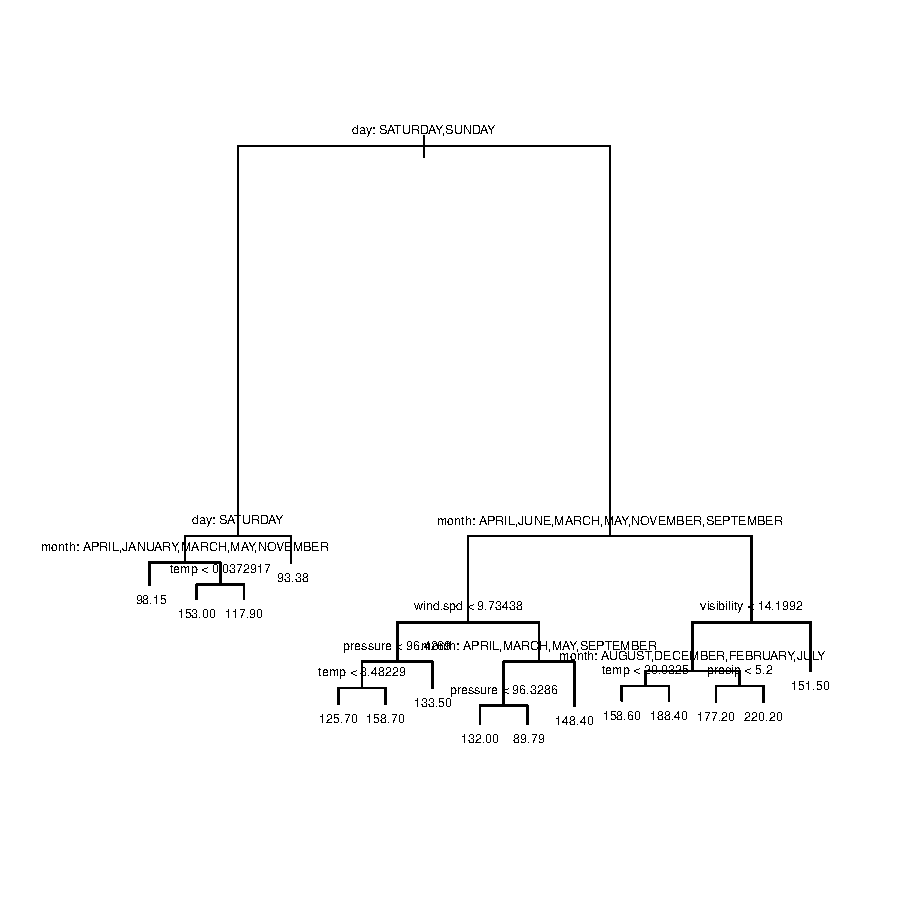
\includegraphics{regression-021}



\begin{Schunk}
\begin{Soutput}
Decision Tree MSE: 1164.874
\end{Soutput}
\end{Schunk}
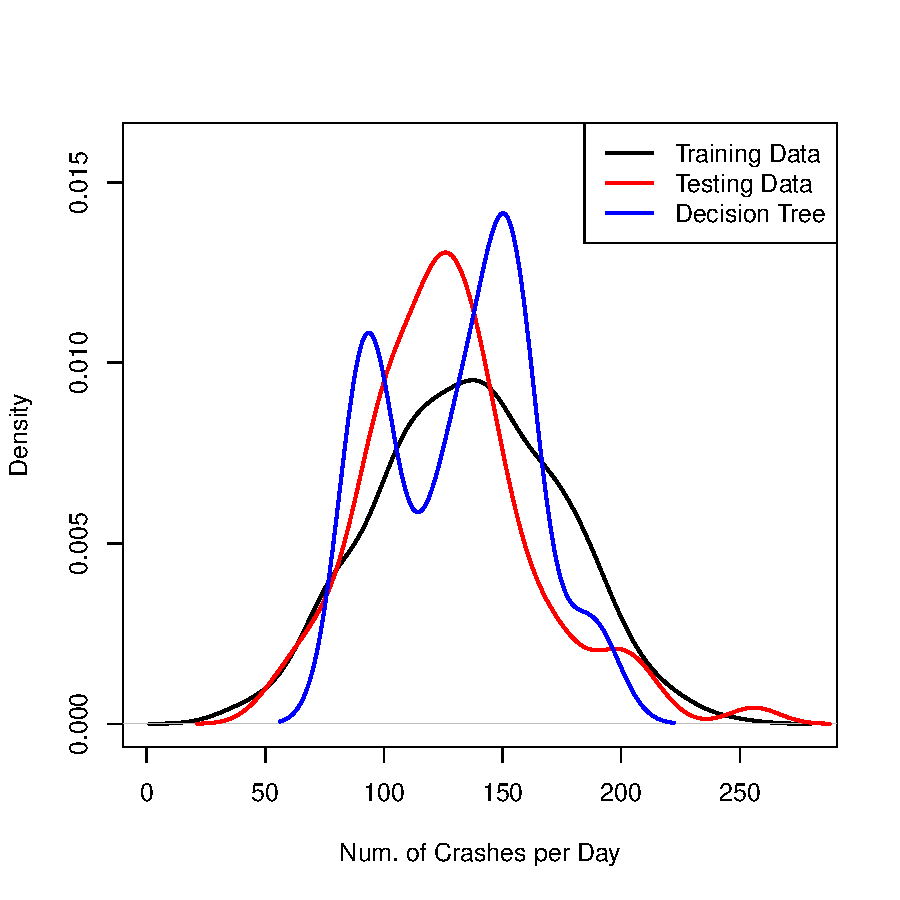
\includegraphics{regression-023}





\pagebreak
\subsection{Random Forest}

\begin{Schunk}
\begin{Soutput}
Call:
 randomForest(formula = crashes ~ month + day + temp + relhum +      precip + wind.dir + wind.spd + visibility + pressure, data = train,      importance = TRUE) 
               Type of random forest: regression
                     Number of trees: 500
No. of variables tried at each split: 3

          Mean of squared residuals: 837.889
                    % Var explained: 44.3
\end{Soutput}
\end{Schunk}


\begin{Schunk}
\begin{Soutput}
Random Forest MSE: 1017.569
\end{Soutput}
\end{Schunk}
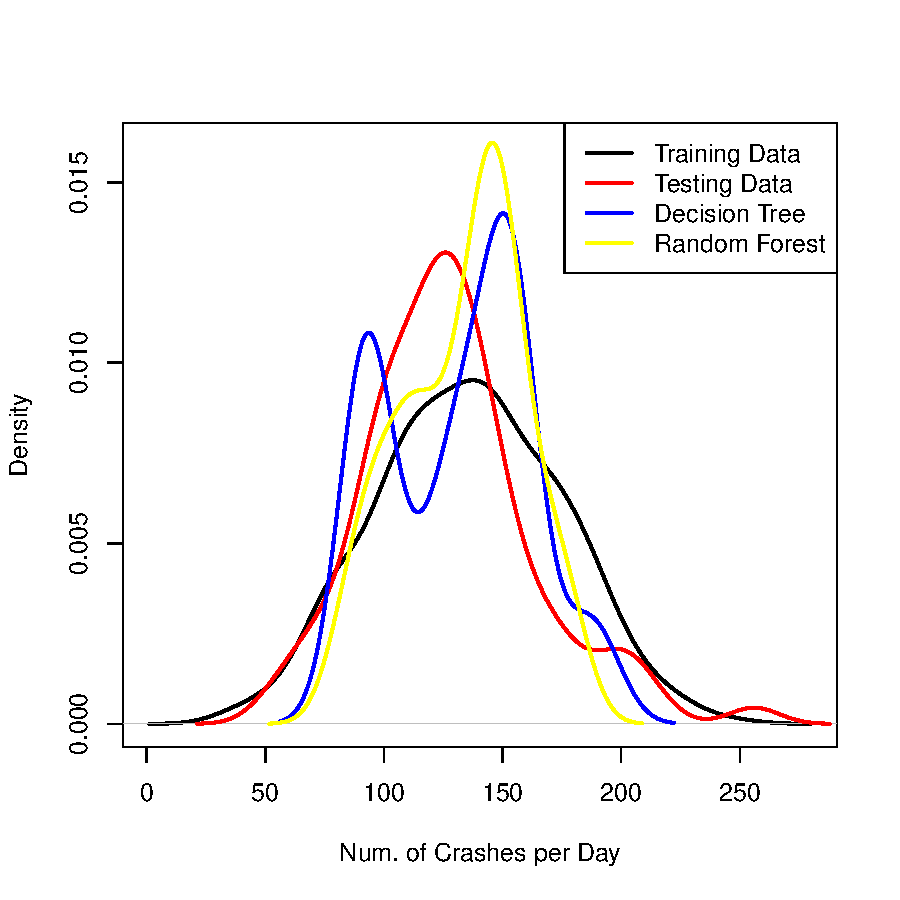
\includegraphics{regression-025}





\pagebreak
\subsection{Boosting}

\begin{Schunk}
\begin{Soutput}
Distribution not specified, assuming gaussian ...
\end{Soutput}
\begin{Soutput}
                  var   rel.inf
month           month 37.449966
day               day 13.487334
wind.dir     wind.dir 10.802975
wind.spd     wind.spd  8.292799
visibility visibility  7.510607
pressure     pressure  6.772252
temp             temp  5.864595
relhum         relhum  5.223828
precip         precip  4.595645
\end{Soutput}
\end{Schunk}

\begin{Schunk}
\begin{Soutput}
Boosting MSE: 1052.224
\end{Soutput}
\end{Schunk}
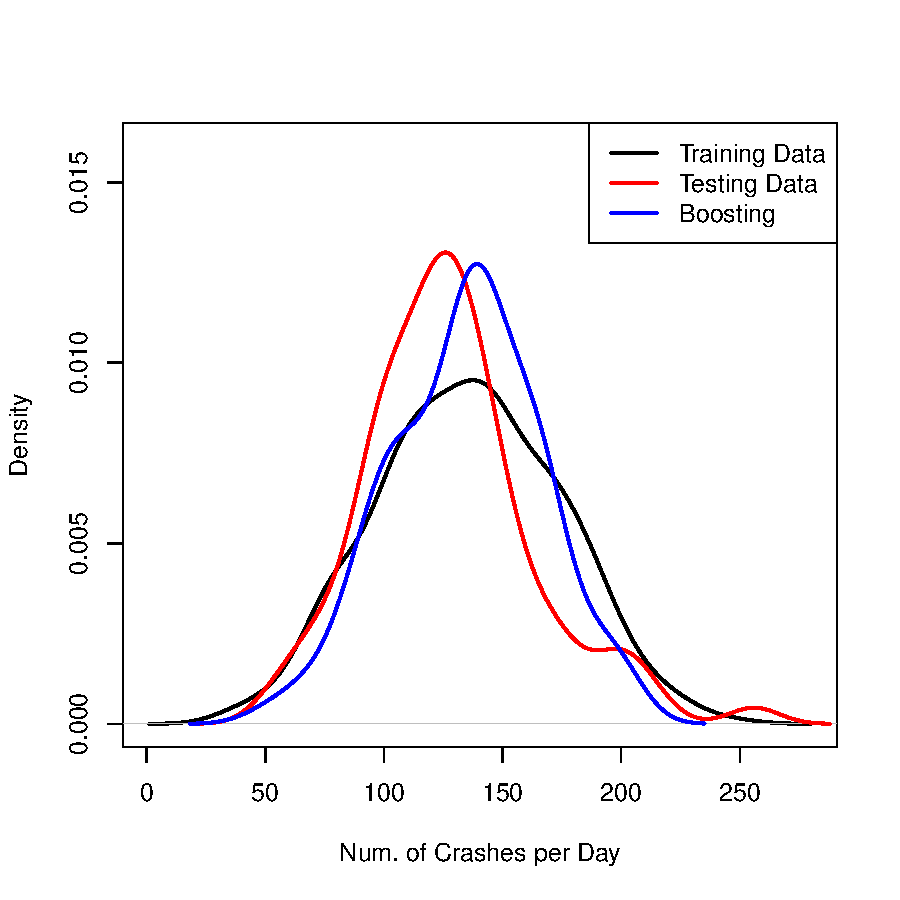
\includegraphics{regression-027}







\pagebreak
\subsection{Regression Summary}


\begin{Schunk}
\begin{Soutput}
All model MSEs:
\end{Soutput}
\begin{Soutput}
      MLR      GLM       NP     Tree       RF Boosting
 1029.308 974.3266 1203.843 1164.874 1017.569 1052.224
\end{Soutput}
\end{Schunk}


\vspace{6pc}

Winner: GLM!









\pagebreak
\section{Predicting Number of Victims}

\subsection{Multiple Linear Regression}

\begin{Schunk}
\begin{Soutput}
Call:
lm(formula = victims ~ month + day + wind.spd, data = train, 
    x = TRUE, y = TRUE)

Residuals:
    Min      1Q  Median      3Q     Max 
-28.201  -6.864   0.272   6.680  37.935 

Coefficients:
               Estimate Std. Error t value Pr(>|t|)    
(Intercept)     48.3371     4.1058  11.773  < 2e-16 ***
monthAUGUST     11.2373     3.0844   3.643 0.000314 ***
monthDECEMBER   10.2125     3.2096   3.182 0.001609 ** 
monthFEBRUARY    7.8671     3.0711   2.562 0.010882 *  
monthJANUARY     9.2144     3.1289   2.945 0.003470 ** 
monthJULY       12.3294     3.0452   4.049 6.48e-05 ***
monthJUNE        9.2431     3.0452   3.035 0.002603 ** 
monthMARCH       1.0384     3.0717   0.338 0.735536    
monthMAY         6.1042     3.0446   2.005 0.045825 *  
monthNOVEMBER    5.1081     3.1965   1.598 0.111040    
monthOCTOBER     9.9902     3.1395   3.182 0.001608 ** 
monthSEPTEMBER  10.5302     3.0902   3.408 0.000740 ***
dayMONDAY      -12.5839     2.3256  -5.411 1.24e-07 ***
daySATURDAY    -21.8174     2.3350  -9.344  < 2e-16 ***
daySUNDAY      -25.5786     2.3266 -10.994  < 2e-16 ***
dayTHURSDAY     -7.6391     2.3499  -3.251 0.001275 ** 
dayTUESDAY      -6.6192     2.3290  -2.842 0.004773 ** 
dayWEDNESDAY    -7.3388     2.3275  -3.153 0.001771 ** 
wind.spd        -0.5891     0.3222  -1.828 0.068447 .  
---
Signif. codes:  0 ‘***’ 0.001 ‘**’ 0.01 ‘*’ 0.05 ‘.’ 0.1 ‘ ’ 1

Residual standard error: 11.39 on 316 degrees of freedom
Multiple R-squared:  0.4259,	Adjusted R-squared:  0.3932 
F-statistic: 13.02 on 18 and 316 DF,  p-value: < 2.2e-16
\end{Soutput}
\end{Schunk}

\begin{Schunk}
\begin{Soutput}
MLR MSE: 153.6082
\end{Soutput}
\end{Schunk}
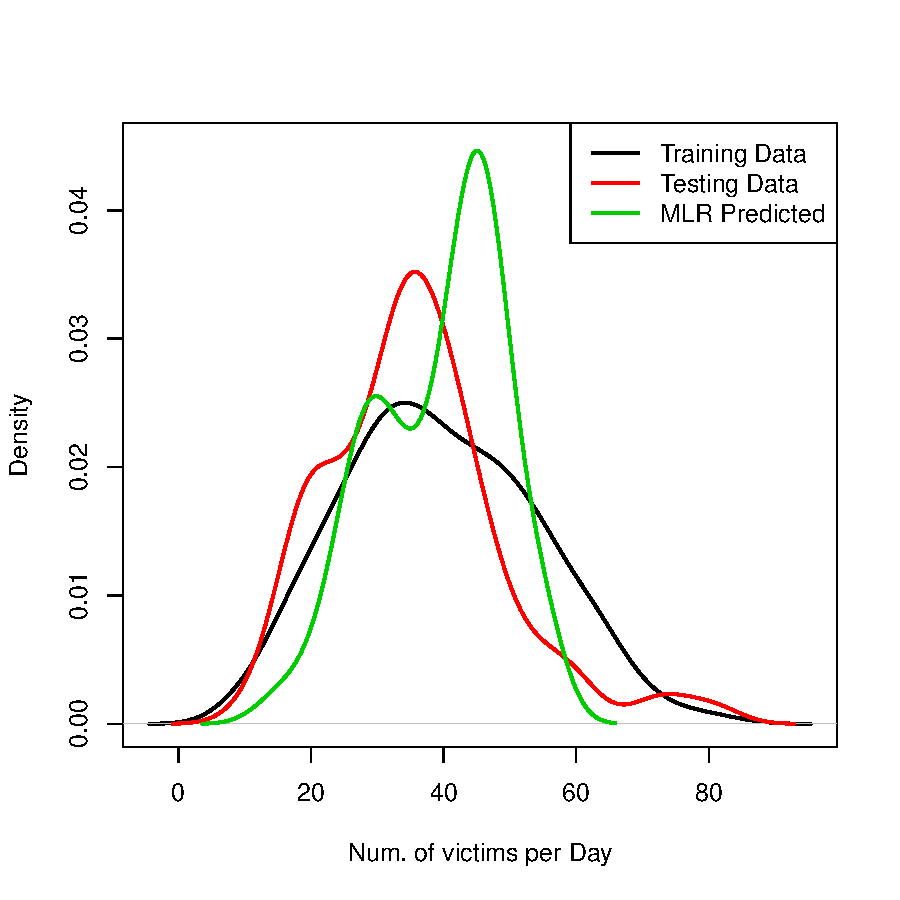
\includegraphics{regression-030}



\begin{Schunk}
\begin{Soutput}
Consistent Model Specification Test
Parametric null model: lm(formula = crashes ~ month + day + temp + relhum +
                          precip + wind.dir + wind.spd + visibility + pressure,
                          data = train, x = TRUE, y = TRUE)
Number of regressors: 9
IID Bootstrap (399 replications)

Test Statistic ‘Jn’: 2.125212	P Value: 0.0075188 **
---
Signif. codes:  0 '***' 0.001 '**' 0.01 '*' 0.05 '.' 0.1 ' ' 1
Null of correct specification is rejected at the 1% level
\end{Soutput}
\end{Schunk}




\pagebreak
\subsection{Generalized Linear Model}


\begin{Schunk}
\begin{Soutput}
Call:
glm(formula = victims ~ month + day + temp + relhum + precip + 
    wind.dir + wind.spd + visibility + pressure, family = gaussian(link = "identity"), 
    data = train)

Deviance Residuals: 
    Min       1Q   Median       3Q      Max  
-29.597   -7.378    0.171    7.247   39.637  

Coefficients:
                Estimate Std. Error t value Pr(>|t|)    
(Intercept)    383.54765  218.89064   1.752 0.080722 .  
monthAUGUST     14.79288    5.51660   2.682 0.007721 ** 
monthDECEMBER   10.36465    5.28669   1.961 0.050830 .  
monthFEBRUARY    3.54993    5.67013   0.626 0.531726    
monthJANUARY     7.31513    5.67695   1.289 0.198510    
monthJULY       17.86761    5.71119   3.129 0.001924 ** 
monthJUNE       13.82776    4.60435   3.003 0.002889 ** 
monthMARCH      -0.98606    3.78617  -0.260 0.794699    
monthMAY         9.30472    4.03556   2.306 0.021788 *  
monthNOVEMBER    6.15255    4.53793   1.356 0.176147    
monthOCTOBER    12.42884    3.70083   3.358 0.000882 ***
monthSEPTEMBER  14.63639    4.17346   3.507 0.000520 ***
dayMONDAY      -12.67408    2.39423  -5.294 2.27e-07 ***
daySATURDAY    -21.74037    2.35150  -9.245  < 2e-16 ***
daySUNDAY      -25.43063    2.35661 -10.791  < 2e-16 ***
dayTHURSDAY     -7.89874    2.36442  -3.341 0.000938 ***
dayTUESDAY      -6.87792    2.36327  -2.910 0.003872 ** 
dayWEDNESDAY    -7.52565    2.34645  -3.207 0.001480 ** 
temp            -0.57623    0.39413  -1.462 0.144744    
relhum          -0.19986    0.13670  -1.462 0.144754    
precip           0.02343    0.17298   0.135 0.892338    
wind.dir         0.34939    0.34815   1.004 0.316375    
wind.spd        -0.98698    0.39037  -2.528 0.011958 *  
visibility      -0.69167    0.59765  -1.157 0.248031    
pressure        -3.21530    2.25158  -1.428 0.154294    
---
Signif. codes:  0 ‘***’ 0.001 ‘**’ 0.01 ‘*’ 0.05 ‘.’ 0.1 ‘ ’ 1

(Dispersion parameter for gaussian family taken to be 129.5969)

    Null deviance: 71422  on 334  degrees of freedom
Residual deviance: 40175  on 310  degrees of freedom
AIC: 2606.3

Number of Fisher Scoring iterations: 2
\end{Soutput}
\end{Schunk}


\begin{Schunk}
\begin{Soutput}
GLM MSE: 142.8508
\end{Soutput}
\end{Schunk}
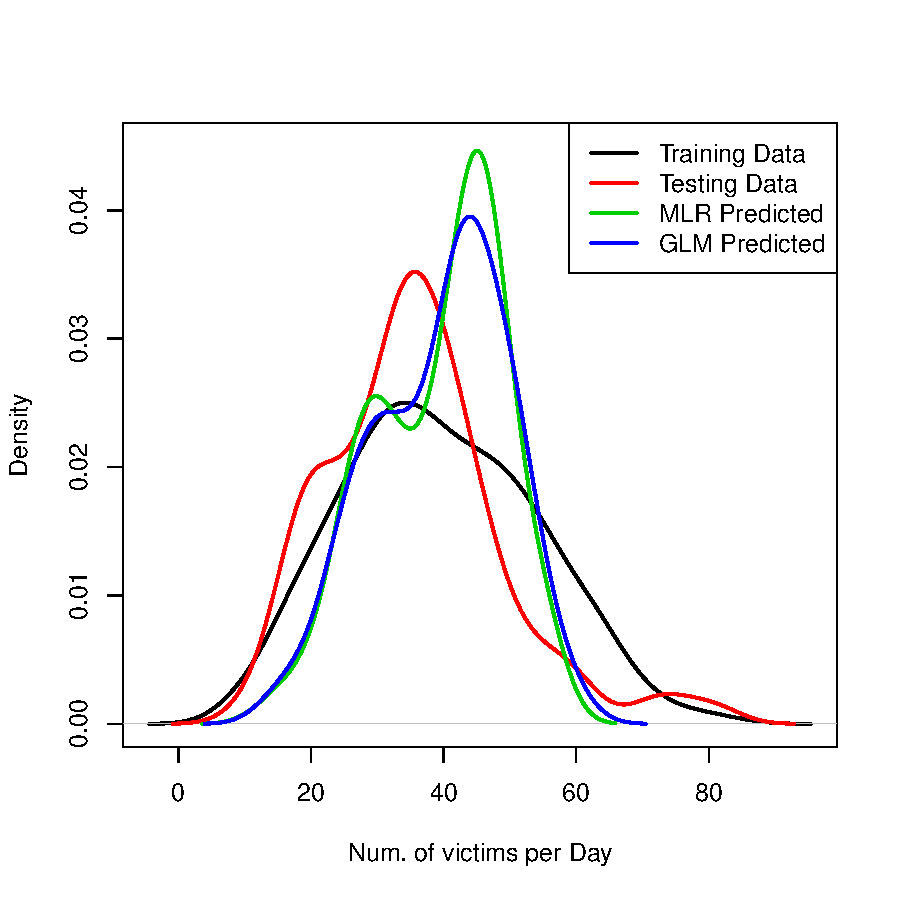
\includegraphics{regression-034}





\pagebreak
\subsection{Non-parametric Approach}

\begin{Schunk}
\begin{Soutput}
Kernel Regression Significance Test
Type I Test with IID Bootstrap (399 replications, Pivot = TRUE, joint = FALSE)
Explanatory variables tested for significance:
month (1), day (2), temp (3), relhum (4), precip (5), wind.dir (6), wind.spd (7), visibility (8), pressure (9)

                 month       day     temp  relhum   precip wind.dir wind.spd
Bandwidth(s): 0.916666 0.4512622 15.01095 11.0829 9.474667  5925261 11.88198
              visibility pressure
Bandwidth(s):   52101772  3255838

Individual Significance Tests
P Value: 
month      0.0025063 ** 
day        < 2.22e-16 *** 
temp       0.0075188 ** 
relhum     0.7969925  
precip     0.0350877 * 
wind.dir   0.1679198  
wind.spd   0.0050125 ** 
visibility 0.0225564 * 
pressure   0.2080201 
---
Signif. codes:  0 '***' 0.001 '**' 0.01 '*' 0.05 '.' 0.1 ' ' 1
\end{Soutput}
\begin{Soutput}
Non-parametric MSE: 170.7991
\end{Soutput}
\end{Schunk}
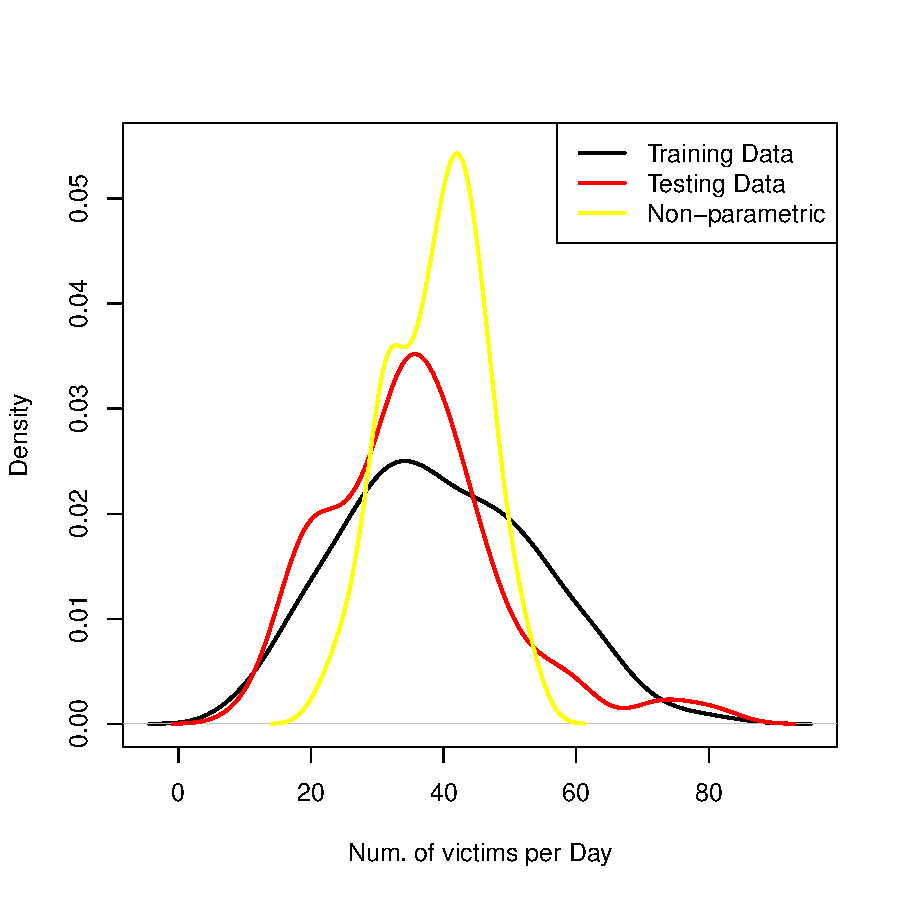
\includegraphics{regression-035}


\pagebreak
\subsection{Decision Tree}

\begin{Schunk}
\begin{Soutput}
Regression tree:
tree(formula = victims ~ month + day + temp + relhum + precip + 
    wind.dir + wind.spd + visibility + pressure, data = train)
Variables actually used in tree construction:
[1] "day"      "month"    "relhum"   "wind.spd" "pressure"
Number of terminal nodes:  13 
Residual mean deviance:  111.3 = 35840 / 322 
Distribution of residuals:
   Min. 1st Qu.  Median    Mean 3rd Qu.    Max. 
-23.770  -7.331  -0.686   0.000   6.606  45.230 
\end{Soutput}
\end{Schunk}
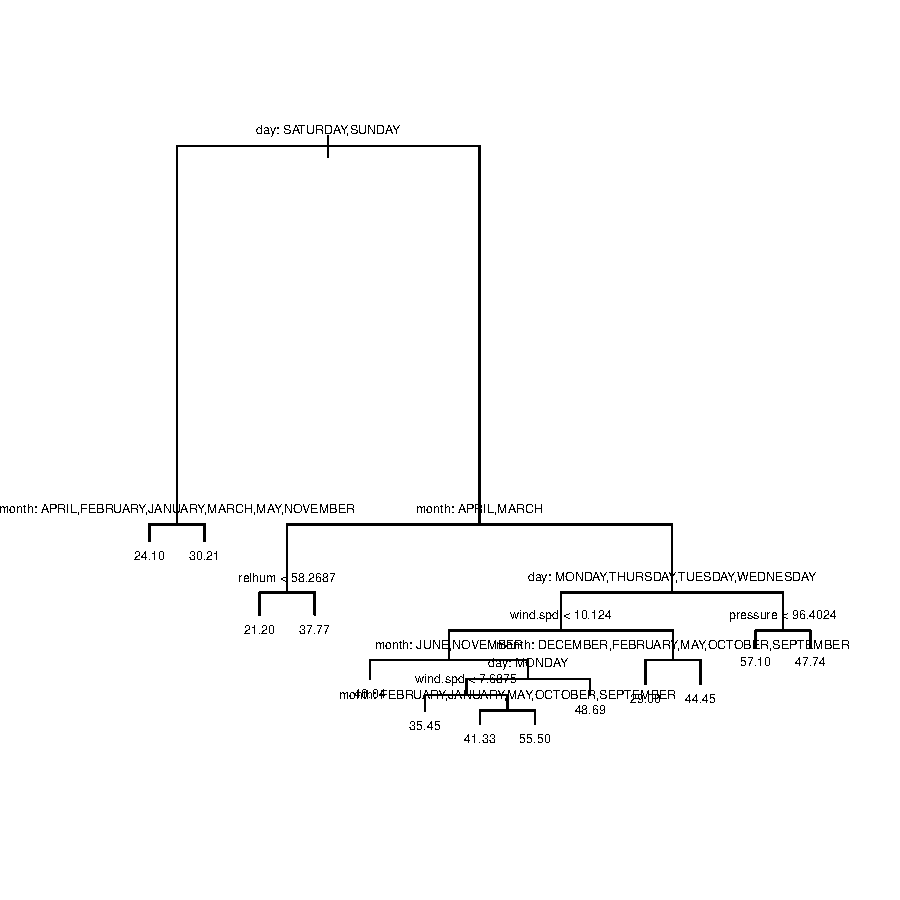
\includegraphics{regression-036}



\begin{Schunk}
\begin{Soutput}
Decision Tree MSE: 180.8277
\end{Soutput}
\end{Schunk}
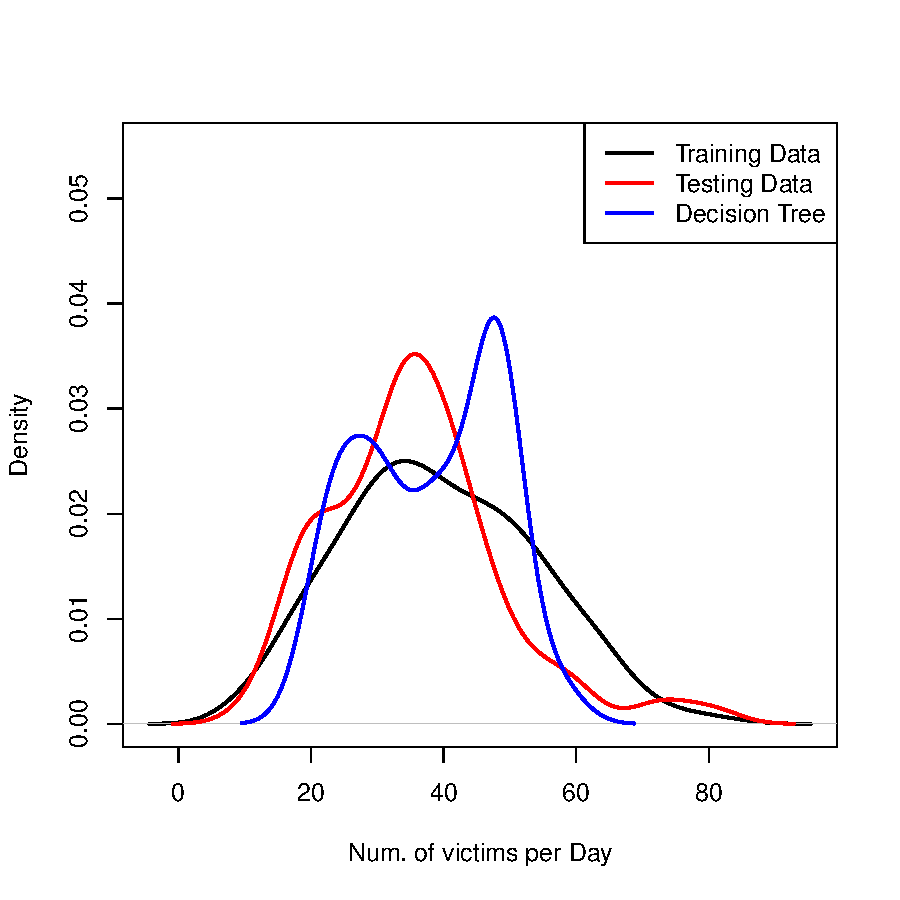
\includegraphics{regression-038}





\pagebreak
\subsection{Random Forest}

\begin{Schunk}
\begin{Soutput}
Call:
 randomForest(formula = victims ~ month + day + temp + relhum +      precip + wind.dir + wind.spd + visibility + pressure, data = train,      importance = TRUE) 
               Type of random forest: regression
                     Number of trees: 500
No. of variables tried at each split: 3

          Mean of squared residuals: 142.6944
                    % Var explained: 33.07
\end{Soutput}
\end{Schunk}


\begin{Schunk}
\begin{Soutput}
Random Forest MSE: 152.5664
\end{Soutput}
\end{Schunk}
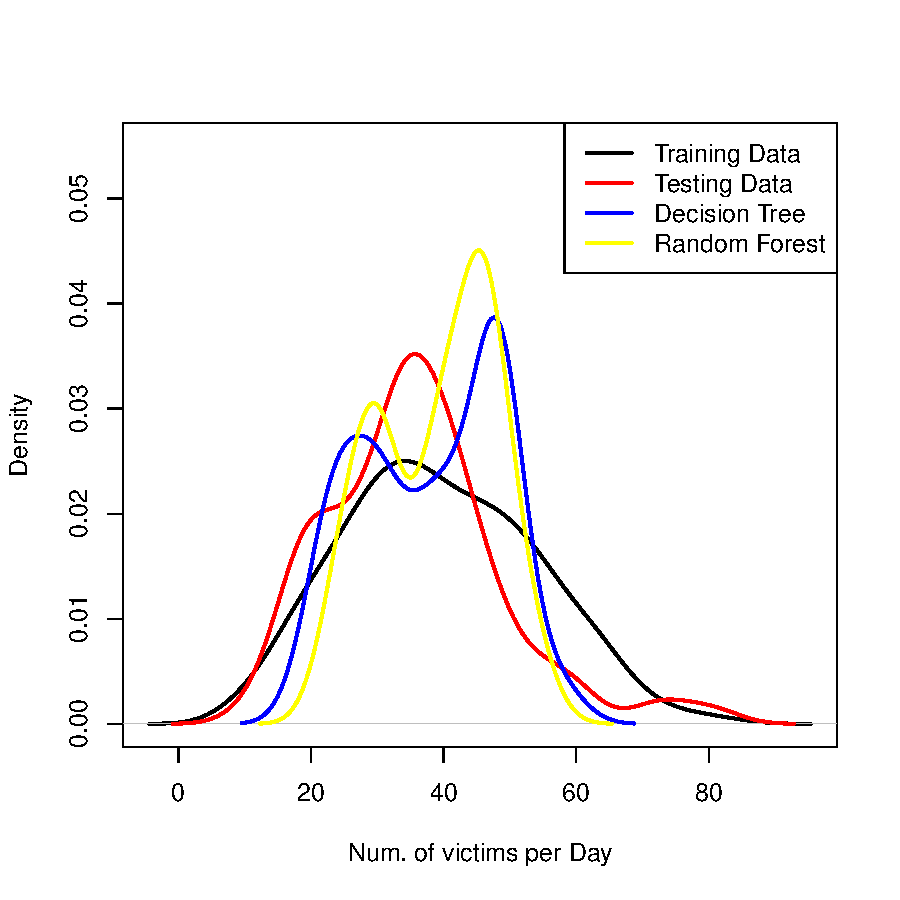
\includegraphics{regression-040}





\pagebreak
\subsection{Boosting}

\begin{Schunk}
\begin{Soutput}
Distribution not specified, assuming gaussian ...
\end{Soutput}
\begin{Soutput}
                  var   rel.inf
month           month 40.877423
day               day 12.957957
pressure     pressure  9.455169
wind.dir     wind.dir  9.081652
visibility visibility  6.599191
wind.spd     wind.spd  6.451126
temp             temp  5.749958
relhum         relhum  4.830842
precip         precip  3.996683
\end{Soutput}
\end{Schunk}

\begin{Schunk}
\begin{Soutput}
Boosting MSE: 143.6589
\end{Soutput}
\end{Schunk}
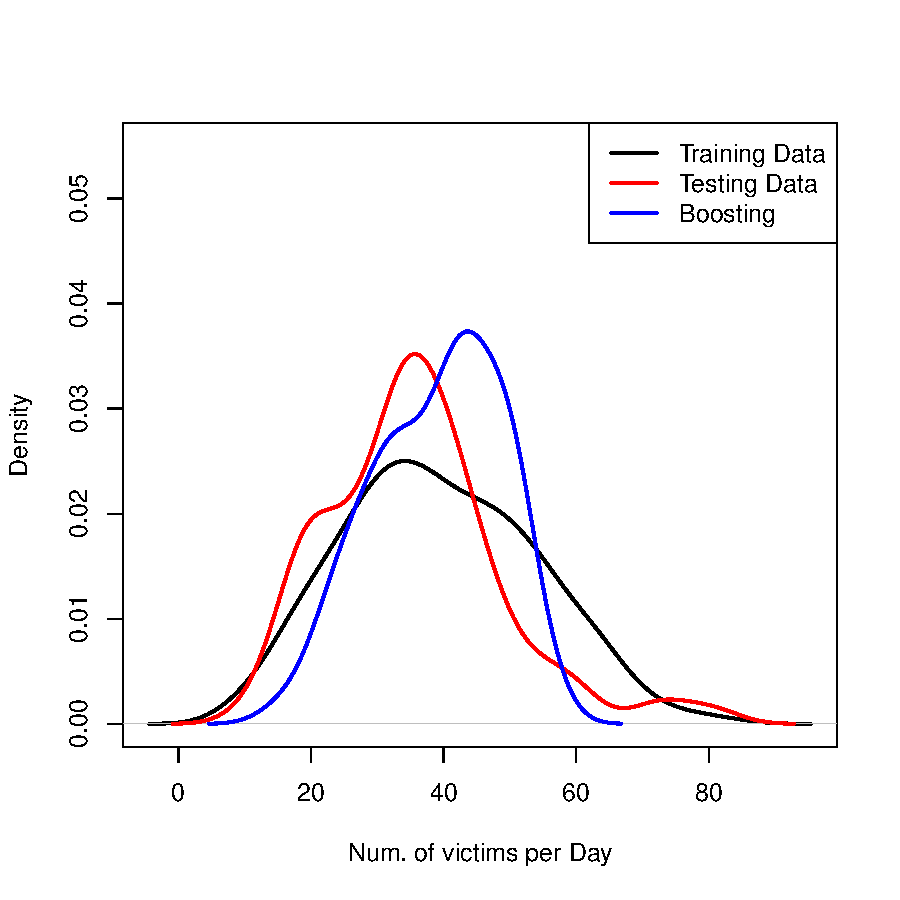
\includegraphics{regression-042}







\pagebreak
\subsection{Regression Summary}


\begin{Schunk}
\begin{Soutput}
All model MSEs:
\end{Soutput}
\begin{Soutput}
      MLR      GLM       NP     Tree       RF Boosting
 153.6082 142.8508 170.7991 180.8277 152.5664 143.6589
\end{Soutput}
\end{Schunk}


\vspace{6pc}


Winner: GLM (again)!






\pagebreak
\section{Answering Hypotheses}

\subsection{Visibility on a given day will be inversely correlated with \# of crashes per day.}

This is true. The GLM (with outlier removed) shows a statistically significant coefficient estimate of -4.1926, meaning that visibility and \# of crashes per day is, indeed, inversely related. 

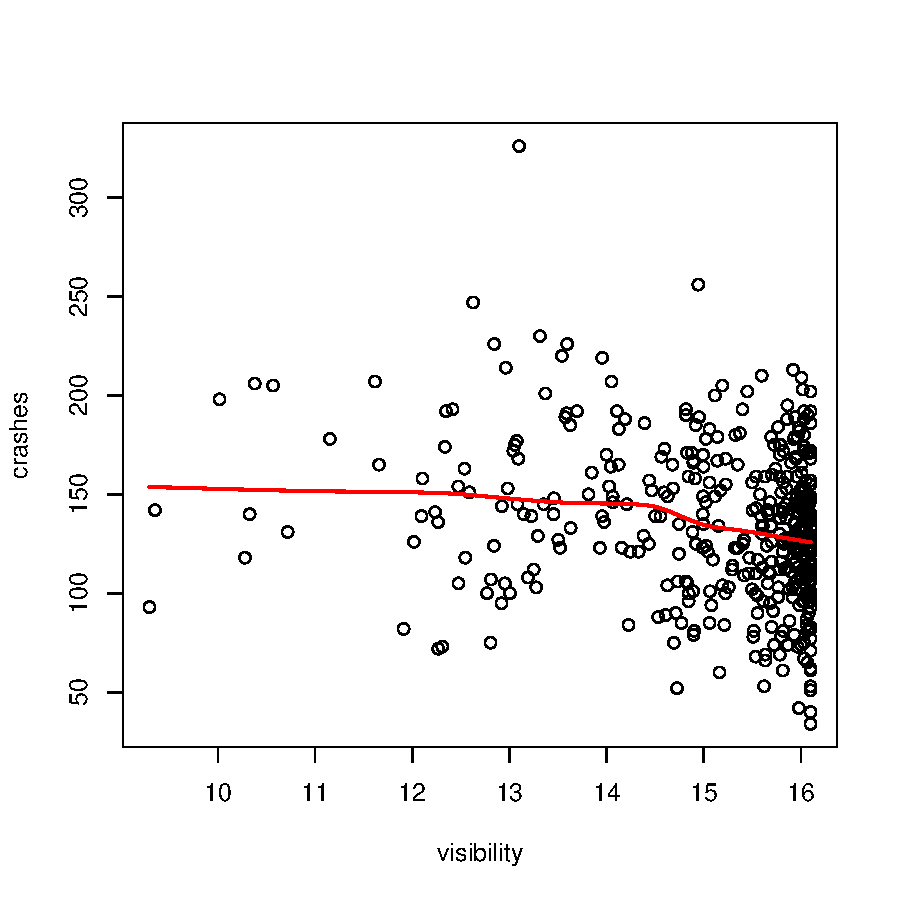
\includegraphics{regression-044}


\pagebreak
\subsection{Temperature will have a weak correlation with \# of crashes per day (people drive more recklessly in the summer? also tourism = more traffic in summer).}


This is false. The GLM shows that temperature is not a statistically significant predictor of the \# of crashes per day. 

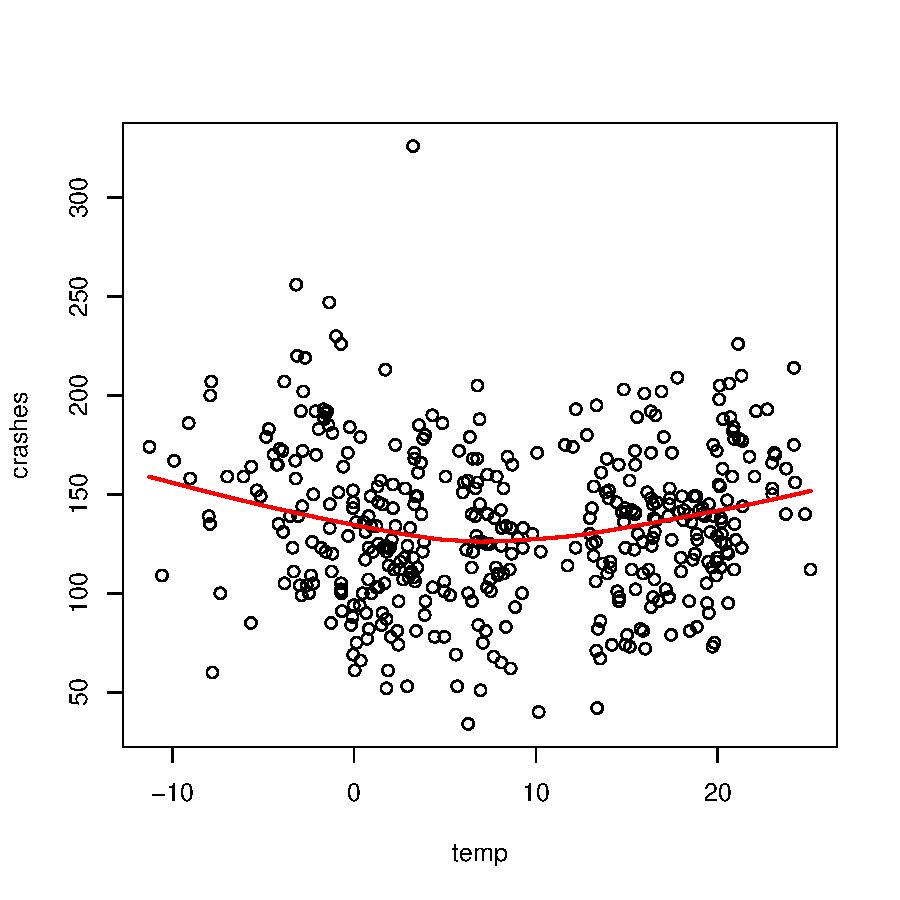
\includegraphics{regression-045}





\pagebreak
\subsection{Precipitation will be correlated with \# of crashes per day.} 

This is unclear. While the GLM does show increasing precipitation to be associated with increasing \# of crashes (0.434), this relationship is not statistically significant (p=0.332). Perhaps with more data (or if the current data was not anonymized), this trend would be confirmed. 

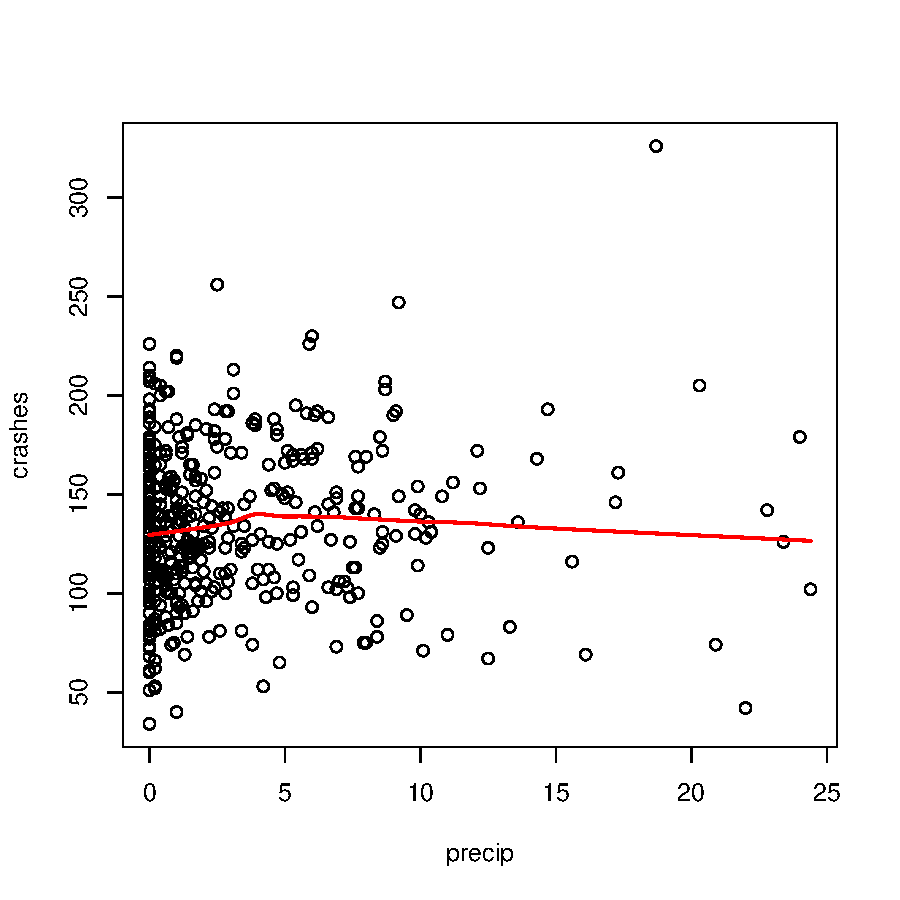
\includegraphics{regression-046}



\pagebreak
\subsection{Summer will have more crashes involving cyclists and motorcyclists.} 


A cursory glance at the variable investigation document will confirm this. 
\par
We can also cluster the months based on season and perform a proper hypothesis test:

\begin{Schunk}
\begin{Soutput}
Cyclist ANOVA:
\end{Soutput}
\begin{Soutput}
            Df Sum Sq Mean Sq F value  Pr(>F)   
season       3   3539  1179.6   7.714 0.00955 **
Residuals    8   1223   152.9                   
---
Signif. codes:  0 ‘***’ 0.001 ‘**’ 0.01 ‘*’ 0.05 ‘.’ 0.1 ‘ ’ 1
\end{Soutput}
\begin{Soutput}
  Tukey multiple comparisons of means
    95% family-wise confidence level

Fit: aov(formula = bike ~ season, data = kwt)

$season
                   diff        lwr           upr     p adj
Spring-Fall   -13.00000 -45.333361  1.933336e+01 0.5946617
Summer-Fall    14.33333 -18.000028  4.666669e+01 0.5223532
Winter-Fall   -32.33333 -64.666694  2.757948e-05 0.0500002
Summer-Spring  27.33333  -5.000028  5.966669e+01 0.1005671
Winter-Spring -19.33333 -51.666694  1.300003e+01 0.2944622
Winter-Summer -46.66667 -79.000028 -1.433331e+01 0.0073984
\end{Soutput}
\begin{Soutput}
Motorcycle ANOVA:
\end{Soutput}
\begin{Soutput}
            Df Sum Sq Mean Sq F value  Pr(>F)   
season       3   9249    3083   10.04 0.00435 **
Residuals    8   2456     307                   
---
Signif. codes:  0 ‘***’ 0.001 ‘**’ 0.01 ‘*’ 0.05 ‘.’ 0.1 ‘ ’ 1
\end{Soutput}
\begin{Soutput}
  Tukey multiple comparisons of means
    95% family-wise confidence level

Fit: aov(formula = motorcycle ~ season, data = kwt)

$season
                     diff         lwr       upr     p adj
Spring-Fall     0.6666667  -45.146744  46.48008 0.9999604
Summer-Fall    43.3333333   -2.480078  89.14674 0.0638450
Winter-Fall   -35.0000000  -80.813411  10.81341 0.1447832
Summer-Spring  42.6666667   -3.146744  88.48008 0.0681892
Winter-Spring -35.6666667  -81.480078  10.14674 0.1357137
Winter-Summer -78.3333333 -124.146744 -32.51992 0.0026273
\end{Soutput}
\end{Schunk}
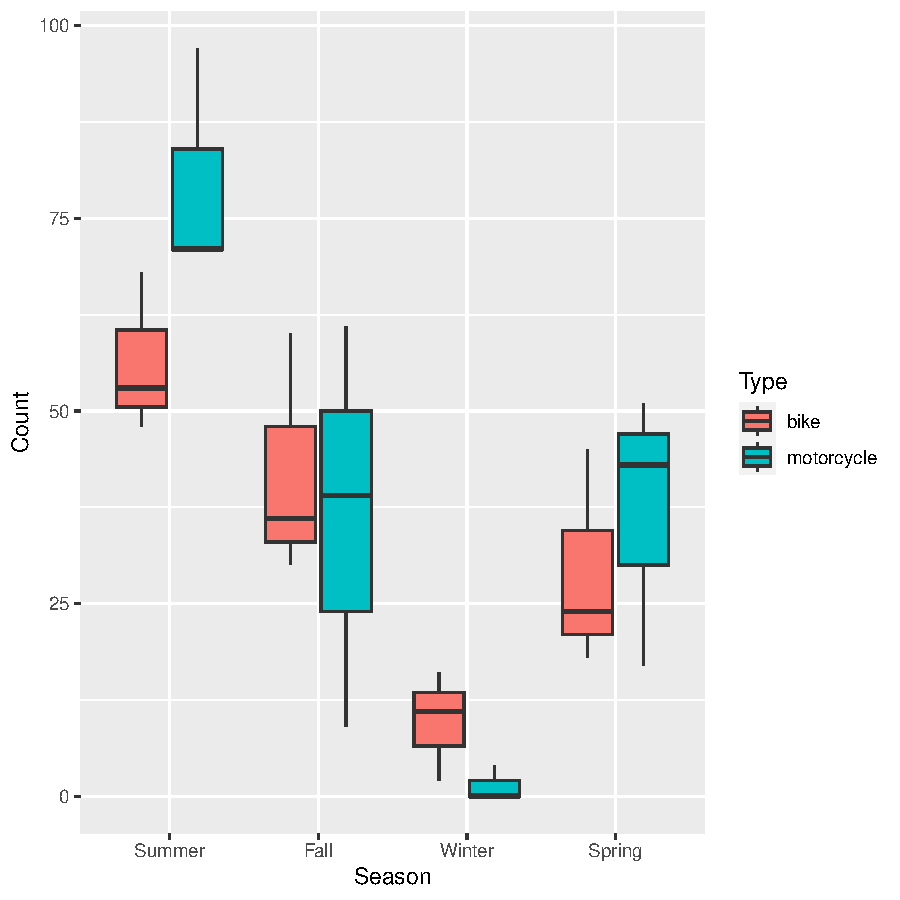
\includegraphics{regression-047}

In summary, yes, summer months have significantly more cyclist and motorcycle accidents (than winter months). 




\pagebreak
\subsection{The number of crashes will increase on weekends when more people are driving under the influence.} 

This is false. By looking at the barplot of accidents throughout the week in the Variable Investigation document, it is clear that there are more crashes on weekdays (Mon-Fri) compared to weekends (Sat-Sun), with the \# of crashes slowly climbing throughout the week. This is the reverse of what was expected. 


\begin{Schunk}
\begin{Soutput}
Reprint of plot from Variable Investigation:
\end{Soutput}
\end{Schunk}
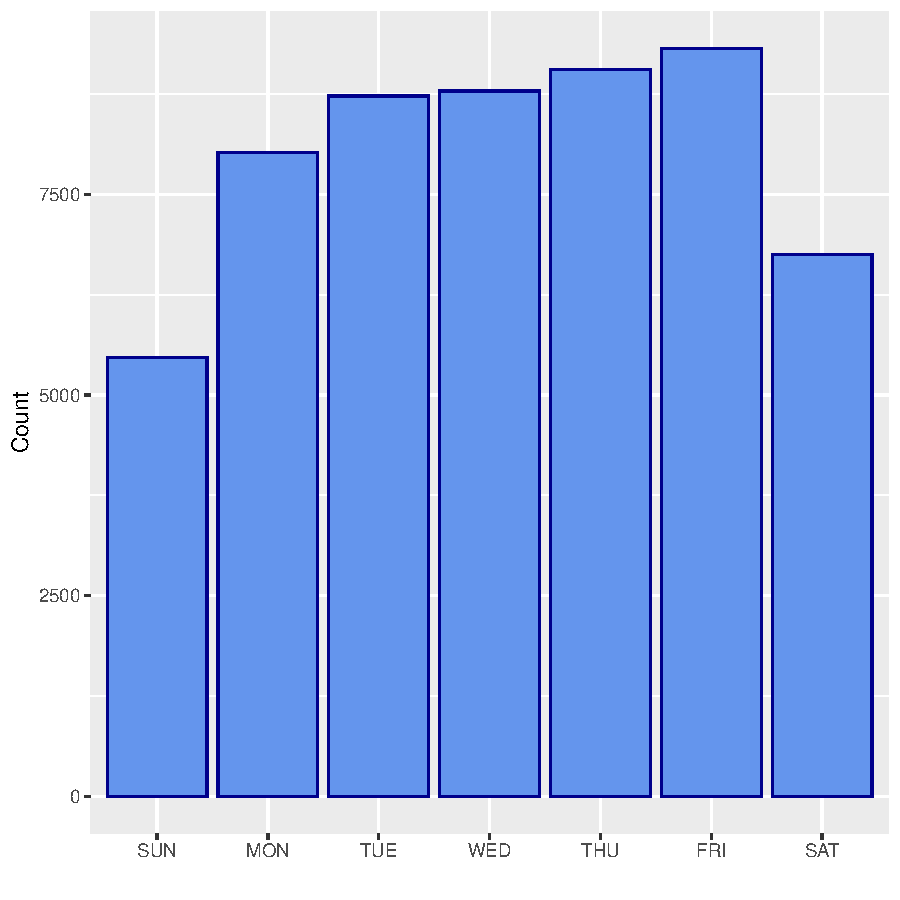
\includegraphics{regression-048}




\pagebreak
\subsection{Fatal, more severe crashes occur proportionately more often at nighttime, as visibility is reduced due to lack of sunlight.} 

By looking at the barplot of accidents throughout the day in the Variable Investigation document, it is clear that more accidents happen during the daytime. However, this is likely due to the fact that more people are driving and are on the roads during the day. Instead, we want to know if nighttime crashes are \textit{more fatal}. 
\par
To determine this, I will give each time block a crash:casualty ratio by dividing the number of fatalities by the number of crashes. This value can then be compared across time categories. I will define 9PM to 6AM as 'nighttime', and 6AM - 9PM as 'daytime'.


\begin{Schunk}
\begin{Soutput}
Crash-Casualty Ratio ANOVA:
\end{Soutput}
\begin{Soutput}
            Df   Sum Sq   Mean Sq F value Pr(>F)
time         1 0.000508 0.0005079   0.206  0.666
Residuals    6 0.014781 0.0024636               
\end{Soutput}
\end{Schunk}
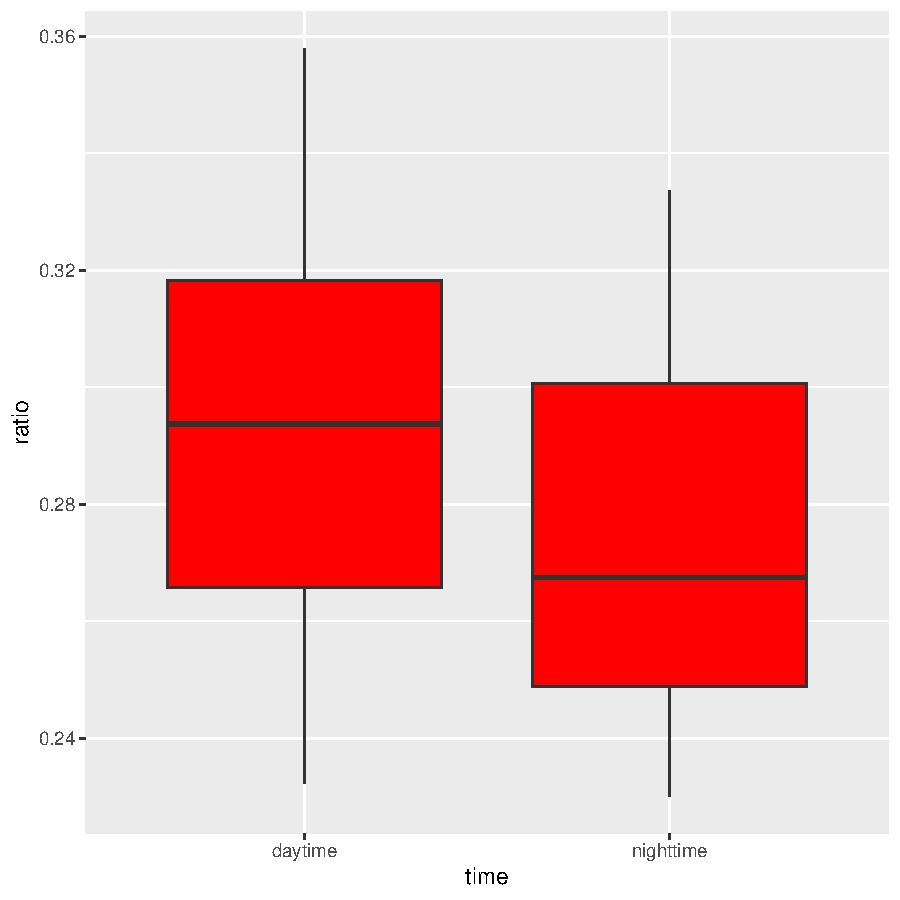
\includegraphics{regression-049}


As you can see, there is no evidence that nighttime accidents are more fatal than daytime ones. 





\pagebreak
\subsection{Single-vehicle crashes should be proportionally higher during adverse weather, especially snow/ice conditions.}

This approach can be similar to the cyclist/motocycle hypothesis above. I will group by season and test for difference using an ANOVA:

\begin{Schunk}
\begin{Soutput}
            Df Sum Sq Mean Sq F value  Pr(>F)   
Season       3 105547   35182   10.09 0.00429 **
Residuals    8  27905    3488                   
---
Signif. codes:  0 ‘***’ 0.001 ‘**’ 0.01 ‘*’ 0.05 ‘.’ 0.1 ‘ ’ 1
\end{Soutput}
\begin{Soutput}
  Tukey multiple comparisons of means
    95% family-wise confidence level

Fit: aov(formula = Count ~ Season, data = single)

$Season
                    diff        lwr       upr     p adj
Spring-Fall   -175.00000 -329.42658 -20.57342 0.0275845
Summer-Fall    -51.66667 -206.09325 102.75991 0.7152015
Winter-Fall     83.66667  -70.75991 238.09325 0.3674538
Summer-Spring  123.33333  -31.09325 277.75991 0.1240470
Winter-Spring  258.66667  104.24009 413.09325 0.0029922
Winter-Summer  135.33333  -19.09325 289.75991 0.0874337
\end{Soutput}
\end{Schunk}
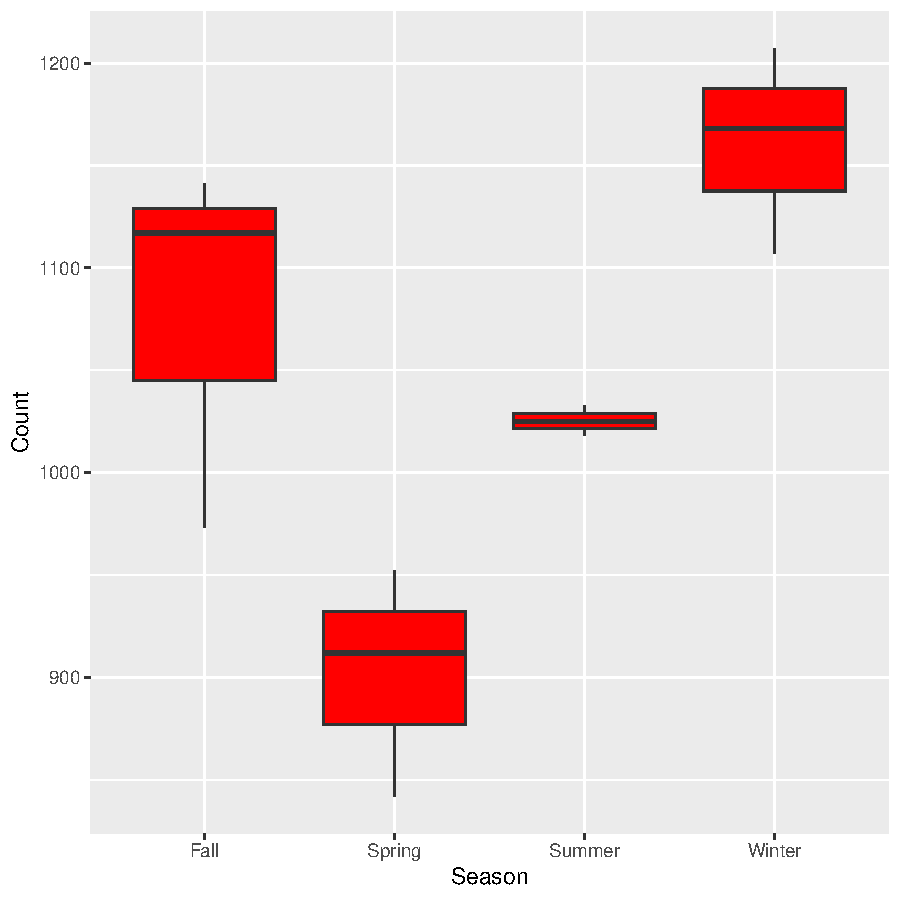
\includegraphics{regression-050}


It appears that most single vehicle collisions occur in the fall and winter, which seems to confirm our hypothesis. However, spring has the least, whereas we have predicted summer to have the least. The winter-summer comparison barely fails to reject (p=0.087), making this hypothesis unclear. 






\end{document}
